\documentclass[aspectratio=169,fleqn]{beamer}
\usepackage{spc}
\usepackage{graphicx}
\begin{document}

\begin{frame}
  \title{\vspace{-5ex}\darkblue Scoping the next stock assessment
    platform\\[2ex]
    \it\large\darkgray
    Project 123 progress update and outline of options}
  \author{\vspace{-10ex}\darkgray\bf
    Arni Magnusson, Nick Davies,\\[0.5ex]
    Graham Pilling, Paul Hamer}
  \date{\darkgreen WCPFC Scientific Committee Meeting (SC20)\\[0.5ex]
    Manila, 14 August 2024}
  \titlepage
\end{frame}

% ______________________________________________________________________________

\begin{frame}{Overview}
  \begin{itemize}
    \item[] {\bf\darkblue Introduction} \comment{background, project outline,
      existing software, new development}\\[5ex]
    \item[] {\bf\darkblue Possible Tasks} \comment{migrate assessments to
      existing software, model exploration,\\
      \h{19.5ex}software development}\\[5ex]
    \item[] {\bf\darkblue Timeline} \comment{PAW 2024, expert meeting 2024,
      workshops 2024--2026,\\
      \h{13ex}launching the main project}\\[5ex]
    \item[] {\bf\darkblue Required Resources} \comment{collaboration with other
      tuna RFMOs,\\
      \h{25.3ex}SPC staff positions \& consultants}\\[1ex]
  \end{itemize}
\end{frame}

% ______________________________________________________________________________

\begin{frame}{The need to to migrate to new software}
  \begin{itemize}
    \item[] MULTIFAN-CL (MFCL) has been used in SPC tuna assessments since
    1990s\\[4ex]
    \item[] MFCL team (Dave Fournier, John Hampton, Nick Davies) retiring in the
    2020s\\[4ex]
    \item[] Development of new features is slowing down\\[4ex]
    \item[] Resources are being allocated to succession plans\\[2ex]
  \end{itemize}
\end{frame}

% ______________________________________________________________________________

\begin{frame}{Migrating all MFCL assessments to other platforms}
  \textbf{\darkgreen Shared} process, {\darkgreen\bf continuous} communications,
  {\darkgreen\bf adaptive} strategy\\[3ex]
  \begin{itemize}
    \item[] {\blue\bf WCPFC} ~--~ guidance\\[2ex]
    \item[] {\blue\bf SPC} ~--~ conduct and coordinate the work\\[4ex]
  \end{itemize}
  Also involved: other tuna RFMOs and various research labs\\[4ex]
  Possibly different software platforms for different stocks\\[4ex]
\end{frame}

% ______________________________________________________________________________

\begin{frame}{Project outline}
  This scoping project is scheduled from 1 Feb 2024 to 31 Dec 2026. It
  will:\\[3ex]
  \begin{itemize}
    \item[] Evaluate features and capabilities that will be important in future
    tuna assessments\\[3ex]
    \item[] Explore fitting models to tuna data using existing software
    platforms\\[3ex]
    \item[] Guide decisions on what kind of new software development will be
    required\\[3ex]
    \item[] Establish collaboration with tuna RFMOs and research labs to achieve
    these goals\\[3ex]
  \end{itemize}
\end{frame}

% ______________________________________________________________________________

\begin{frame}{Possible tasks for SPC to prioritize}
  Subject to SC advice and funding approvals by WCPFC:\\[3ex]
  \begin{itemize}
    \item {\orange\it Migrate assessments to existing software}\\[2ex]
    \item {\orange\it Model exploration using existing software}\\[2ex]
    \item {\orange\it Extend existing software}\\[2ex]
    \item {\orange\it Design and develop new software for tuna
      assessments}\\[2ex]
  \end{itemize}
\end{frame}

% ______________________________________________________________________________

\begin{frame}{2024 project activities}
  \begin{itemize}
    \item[] Scoping project launched (Feb)\\[3ex]
    \item[] Pre-assessment workshop (Mar)\\[3ex]
    \item[] International expert meeting (May--Jun)\\[3ex]
    \item[] SC20 discussion (Aug)\\[3ex]
    \item[] Developer workshop (Aug--Sep)\\[3ex]
    \item[] Follow up with tuna RFMOs and research labs (Oct-Dec)\\[2ex]
  \end{itemize}
\end{frame}

% ______________________________________________________________________________

\begin{frame}{International expert meeting 2024}
  \begin{itemize}
    \item[] Invited stock assessment and software development experts from
    around the world\\
    \comment{tuna RFMOs and various research labs}\\
    \comment{stock assessment software projects, relevant programming
      environments}\\[4ex]
    \item[] Around 40 participants, two sessions covering European and N
    American time zones\\[4ex]
    \item[] Objectives: communicate, discuss, seek advice and
    collaboration\\[4ex]
    \item[] Outcomes: {\darkgreen\bf recommendations}, expressed interest in
    {\darkgreen\bf collaboration} among scientists\\[2ex]
  \end{itemize}
\end{frame}

% ______________________________________________________________________________

\begin{frame}{Timeline}
  \begin{itemize}
    \item[] 2024 \quad Scoping project launched\\[1ex]
    \item[] \phantom{2024} \quad Pre-assessment workshop\\[1ex]
    \item[] \phantom{2024} \quad International expert meeting\\[1ex]
    \item[] \phantom{2024} \quad SC20 discussion\\[3ex]
    \item[] 2024--2026\quad Workshops\\[3ex]
    \item[] 2024--2026\quad Launching the {\darkgreen\bf main project}\\[3ex]
  \end{itemize}
\end{frame}

% ______________________________________________________________________________

\begin{frame}{The main project}
  The current annual budget of project 123 is sufficient for {\darkgreen\bf
    scoping the needs},\\[0.5ex]
  identifying current software platforms, reaching out to the scientific
  community\\[0.5ex]
  for consultation, and to conduct occasional workshops to strengthen\\[0.5ex]
  collaboration ties and initial explorations.\\[5ex]
  The goal of the {\darkgreen\bf main project}, which could either overlap or
  succeed the scoping project,\\[0.5ex]
  is to test/develop tuna stock assessment software and transition all SPC
  assessments\\[0.5ex]
  from MFCL to other platforms.\\[2ex]
\end{frame}

% ______________________________________________________________________________

\begin{frame}{Scoping project (first line) and main project (next lines)}
  \vspace{1ex}
  ~\h{-3ex}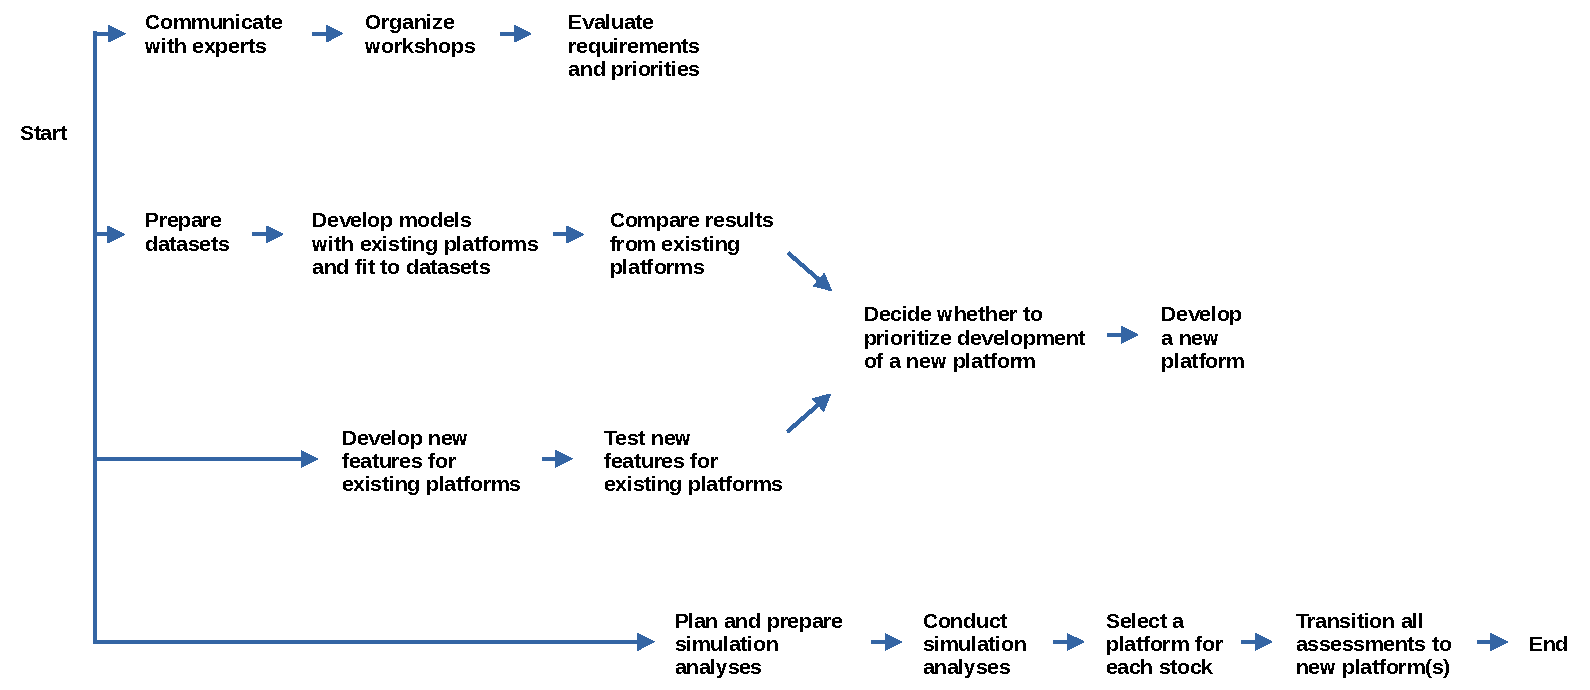
\includegraphics[width=1.05\textwidth]{p123_diagram}
\end{frame}

% ______________________________________________________________________________

\begin{frame}{Required resources}
  The overarching objective of transitioning all WCPFC assessments from
  MULTIFAN-CL\\[0.5ex]
  to other software platforms will require a larger project with
  additional project resources\\[0.5ex]
  beyond the standard service provision agreement for stock assessments, to
  allow some\\[0.5ex]
  staff to focus on model exploration and software development.
\end{frame}

% ______________________________________________________________________________

\begin{frame}{Collaboration with other tuna RFMOs}
  Other tuna RFMOs use primarily Stock Synthesis for tuna assessments,\\[0.5ex]
  a platform that is also expected to be phased out in the not-too-distant
  future.\\[0.5ex]
  Therefore, it would make sense for WCPFC and other tuna RFMOs to
  coordinate\\[0.5ex]
  and collaborate in software succession plans and new software
  development.\\[5ex]
  Ideally, each tuna RFMO could hire/assign one full-time person to the
  project\\[0.5ex]
  for 5 years, or until assessments have been transitioned to the new
  software.\\[4ex]
\end{frame}

% ______________________________________________________________________________

\begin{frame}{SPC staff positions and consultants}
  Compared to the other tuna RFMOs, there is greater urgency for WCPFC\\[0.5ex]
  to move this project forward.\\[4ex]

  Independent of decisions and commitments of the other tuna RFMOs, the\\[0.5ex]
  main project would probably require one staff to be dedicated to this
  work\\[0.5ex]
  initially and, depending on the direction taken, an additional staff or
  consultant\\[0.5ex]
  with software development skills.\\[4ex]

  It is likely that transitioning MFCL assessments to other software is at
  least\\[0.5ex]
  a 5 year proposition.\\[1ex]
\end{frame}

% ______________________________________________________________________________

\begin{frame}{Scientific quality and rate of progress}
  The resources committed to the main project will determine the\\[0.5ex]
  scientific quality of the end result and the number of years it takes\\[0.5ex]
  to transition all SPC assessments from MFCL to other platforms.\\[5ex]
  Now that the first author of MFCL, David Fournier, has retired, it would
  be\\[0.5ex]
  highly beneficial for the project to move relatively fast, before the
  remaining\\[0.5ex]
  MFCL team (John Hampton and Nick Davies) will retire and no longer be\\[0.5ex]
  available for consultation and involvement regarding software design,
  testing\\[0.5ex]
  and technical decisions.
\end{frame}

% ______________________________________________________________________________

\begin{frame}{Summary}
  \begin{itemize}
    \item[] {\bf\darkblue Introduction} \comment{background, project outline,
      existing software, new development}\\[5ex]
    \item[] {\bf\darkblue Possible Tasks} \comment{migrate assessments to
      existing software, model exploration,\\
      \h{19.5ex}software development}\\[5ex]
    \item[] {\bf\darkblue Timeline} \comment{PAW 2024, expert meeting 2024,
      workshops 2024--2026,\\
      \h{13ex}launching the main project}\\[5ex]
    \item[] {\bf\darkblue Required Resources} \comment{collaboration with other
      tuna RFMOs,\\
      \h{25.3ex}SPC staff positions \& consultants}\\[1ex]
  \end{itemize}
\end{frame}

% ______________________________________________________________________________

\begin{frame}{SC20 discussion}
  \begin{itemize}
    \item Whether SPC should migrate upcoming {\darkgreen\bf billfish
      assessments} to Stock Synthesis\\
    \comment{\gray swordfish 2025, striped marlin 2029}\\[4ex]
    \item Select {\darkgreen\bf scoping project} tasks to prioritize in
    2024--2026\\
    \comment{\gray from the list of 10 tasks in the report, or other
      tasks}\\[4ex]
    \item What is needed to launch the {\darkgreen\bf main project} and when\\
    \comment{\gray conducting model exploration and software development, TORs,
      resources}\\[3ex]
  \end{itemize}
\end{frame}

% ______________________________________________________________________________

\begin{frame}{Stock Synthesis}
  \textit{Cons}
  \begin{itemize}
    \item[--] expected to be phased out in the not-too-distant future\\[1ex]
    \item[--] fewer features than MFCL\\[3ex]
  \end{itemize}
  \textit{Pros}
  \begin{itemize}
    \item[+] used by IATTC, IOTC, ICCAT, and ISC (and NOAA, ICES, GFCM,
    etc.)\\[1ex]
    \item[+] facilitates collaboration between the tuna RFMOs, including future
    development\\[1ex]
    \item[+] shortens training time for new SPC staff, makes skills and
    experience transferable\\[1ex]
    \item[+] large user community, relevant for peer reviews and discussing
    technical decisions\\[1ex]
    \item[+] exceptionally complete suite of tools, diagnostics, automated plots
    and tables\\[1ex]
    \item[+] next-generation frameworks will support transitioning from Stock
    Synthesis\\[1ex]
  \end{itemize}
\end{frame}

% ______________________________________________________________________________

\begin{frame}{Recommendations from 2024 international expert meeting}
  \begin{enumerate}
    \item {\darkgreen\bf Tuna} assessment software\\
    \comment{\gray design and develop a model specific for tuna
      assessments}\\[1ex]
    \item {\darkgreen\bf RTMB} programming environment\\
    \comment{\gray lean software development paradigm, maybe a specific model
      for each species}\\[1ex]
    \item {\darkgreen\bf State-space} formulation\\
    \comment{\gray statistically and computationally efficient way to allow
      time-varying processes}\\[1ex]
    \item {\darkgreen\bf Age-length} structure\\
    \comment{\gray explicitly track the population by age and length, if not too
      costly}\\[1ex]
    \item {\darkgreen\bf Simple} models\\
    \comment{\gray short-term staff, young scientists, simple user interface,
      simpler models}\\[1ex]
    \item {\darkgreen\bf Collaboration} between tuna RFMOs\\
    \comment{\gray MFCL and Stock Synthesis in a sunset phase, data analyses
      comparable between RFMOs}\\[1.5ex]
  \end{enumerate}
\end{frame}

% ______________________________________________________________________________

\begin{frame}{Stock assessment software}
  Existing software, ready for multi-region tuna assessments\\[3ex]
  \begin{itemize}
    \item[-] {\darkgreen\bf Stock Synthesis} is used by IATTC, IOTC, and
    ICCAT\\[3ex]
    \item[-] {\darkgreen\bf Gadget} has many features relevant for tuna
    assessments\\[3ex]
    \item[-] {\darkgreen\bf Casal} has many features relevant for tuna
    assessments\\[4ex]
  \end{itemize}
  These could be extended further as needs arise\\[2ex]
\end{frame}

% ______________________________________________________________________________

\begin{frame}{Stock assessment software}
  Software that could be developed further:\\[3ex]
  \begin{itemize}
    \item[-] {\darkgreen\bf sbt} is built around CKMR, currently for
    single-region assessments\\[3ex]
    \item[-] {\darkgreen\bf ALSCL} is a state-space model that fits length
    comps, currently no catches\\[3ex]
    \item[-] {\darkgreen\bf WHAM$\,$\raisebox{0.15ex}{+}$\,$Length} is a
    state-space that fits length comps, currently single-region\\[3ex]
    \item[-] {\darkgreen\bf SAM$\,$\raisebox{0.15ex}{+}$\,$Length} is an early
    exploration of extending SAM to fit length comps\\[3ex]
    \item[-] {\darkgreen\bf Stock Synthesis$\,$\raisebox{0.15ex}{+}$\,$Enhanced
      Tags} is a proposed enhancement of the tag module\\[2ex]
  \end{itemize}
\end{frame}

% ______________________________________________________________________________

\begin{frame}{Stock assessment software}
  Also relevant:\\[4ex]
  \begin{itemize}
    \item[-] {\darkgreen\bf Stock Synthesis$\,$\raisebox{0.15ex}{+}$\,$CKMR} is
    an experimental add-on, not included in core software\\[4ex]
    \item[-] {\darkgreen\bf FIMS}, NOAA project coordinating the development of
    a next-generation framework\\[6ex]
  \end{itemize}
\end{frame}

% ______________________________________________________________________________

\begin{frame}{Possible tasks for SPC to prioritize}
  Subject to SC advice and funding approvals by WCPFC:\\[4ex]
  {\orange\it Migrate assessments to existing software}\\[2ex]
  \begin{enumerate}
    \item Move the {\darkgreen swordfish} assessment to Stock Synthesis\\
    \comment{\gray relatively simple compared to other SPC assessments}\\[3ex]
    \item Move the {\darkgreen striped marlin} assessment to Stock Synthesis\\
    \comment{\gray also relatively simple}\\[3ex]
  \end{enumerate}
  \gray stepwise: previous MFCL diagnostic $\Rightarrow$ catch-conditioned
  MFCL $\Rightarrow$ Stock Synthesis
\end{frame}

% ______________________________________________________________________________

\begin{frame}{Possible tasks for SPC to prioritize}
  Subject to SC advice and funding approvals by WCPFC:\\[3.5ex]
  {\orange\it Model exploration using existing software}\\[2ex]
  \begin{enumerate}\setcounter{enumi}{2}
    \item Explore Casal/Gadget/Stock Synthesis/sbt models for {\darkgreen
      albacore}\\
    \comment{\gray simpler than the other tuna species}\\[3ex]
    \item Explore Casal/Gadget/Stock Synthesis models for original {\darkgreen
      five-region yellowfin} data\\
    \comment{\gray test capabilities of platforms: regions, tags, large number
      of fisheries}\\[3ex]
    \item Explore a variety of models for a simplified {\darkgreen single-region
      yellowfin} tuna dataset\\
    \comment{\gray ALSCL, Casal, Gadget, MFCL, sbt, Stock Synthesis,
      WHAM\raisebox{0.15ex}{+}Length}\\[3ex]
  \end{enumerate}
\end{frame}

% ______________________________________________________________________________

\begin{frame}{Possible tasks for SPC to prioritize}
  Subject to SC advice and funding approvals by WCPFC:\\[3ex]
  {\orange\it Extend existing software}\\[1.5ex]
  \begin{enumerate}\setcounter{enumi}{5}
    \item ALSCL$\,$\raisebox{0.15ex}{+}$\,$Fleets\\
    \comment{\gray Fan Zhang (Shanghai Ocean University) and Nick Davies (SPC
      consultant)}\\[1.5ex]
    \item Stock Synthesis$\,$\raisebox{0.15ex}{+}$\,$Enhanced Tags\\
    \comment{\gray Nicholas Ducharme-Barth, Matthew Vincent (NOAA), and Arni
      Magnusson (SPC)}\\[1.5ex]
    \item WHAM$\,$\raisebox{0.15ex}{+}$\,$Length\\
    \comment{\gray Giancarlo Correa (AZTI) and Arni Magnusson (SPC)}\\[1.5ex]
    \item SAM$\,$\raisebox{0.15ex}{+}$\,$Length\\
    \comment{\gray Anders Nielsen (DTU), Colin Millar (ICES), and Arni Magnusson
      (SPC)}\\[1.5ex]
  \end{enumerate}
\end{frame}

% ______________________________________________________________________________

\begin{frame}{Possible tasks for SPC to prioritize}
  Subject to SC advice and funding approvals by WCPFC:\\[4ex]
  {\orange\it Design and develop new software for tuna assessments}\\[2ex]
  \begin{enumerate}\setcounter{enumi}{9}
    \item Initial explorations using {\darkgreen RTMB}\\
    \comment{\gray Nick Davies (SPC consultant) and Arni Magnusson (SPC)}
  \end{enumerate}
\end{frame}

% ______________________________________________________________________________

\begin{frame}{Project website}
  \centering\small
  \textblue{\url{https://github.com/PacificCommunity/ofp-sam-transition-plan}}
\end{frame}

\end{document}
